
\begin{frame}{VELOCITÀ INFERENZA - DSSD}
    \renewcommand{\thefootnote}{\fnsymbol{footnote}}
    Differenza \emph{Frames-Per-Second (FPS)} medi tra il modello di partenza 
    {\color{red}{\bfseries{\emph{SSD}}}} e il modello proposto {\color{OliveGreen}{\bfseries{\emph{DSSD}}}}. Benchmark\footnotemark[1] svolti con gli acceleratori 
    \emph{TensorRT} e \emph{OpenCV(cuDNN)} su tutte e tre le architetture di riferimento.\\
    \vspace{0.2cm}
    \begin{minipage}{\linewidth}
        \centering
        \begin{minipage}{0.45\linewidth}
            \begin{figure}
                \centering
                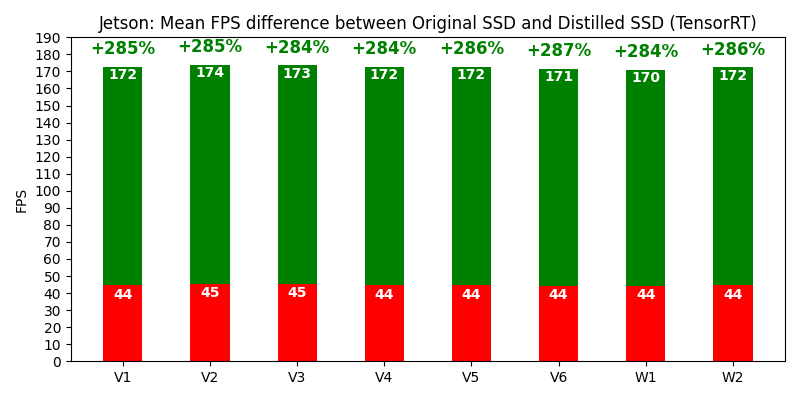
\includegraphics[width = \linewidth]{Mean Difference FPS Jetson TensorRT.png}
                \centering
                \vspace{-0.7cm} 
                \caption{{\bfseries{\emph{Jetson Nano (TensorRT)}}}}
            \end{figure}
        \end{minipage}
        \begin{minipage}{0.45\linewidth}
            \begin{figure}
                \centering
                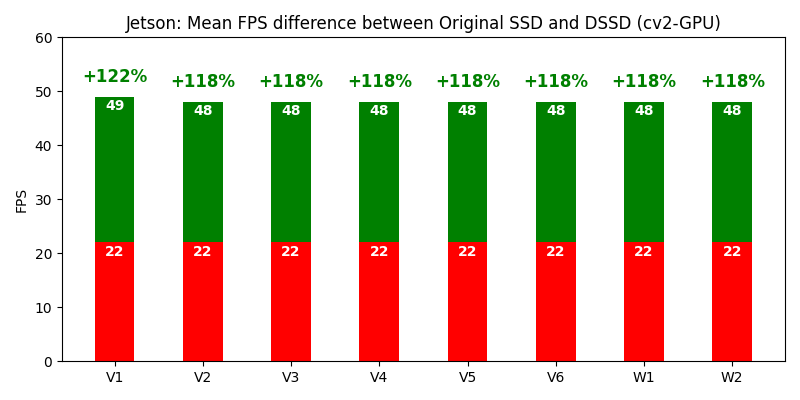
\includegraphics[width = \linewidth]{Difference FPS Jetson cv2 Cuda.png}
                \centering
                \vspace{-0.7cm} 
                \caption{{\bfseries{\emph{Jetson Nano (OpenCV - GPU)}}}}
            \end{figure}
        \end{minipage}
    \end{minipage}
    \begin{minipage}{\linewidth}
        \centering
        \begin{minipage}{0.45\linewidth}
            \begin{figure}
                \centering
                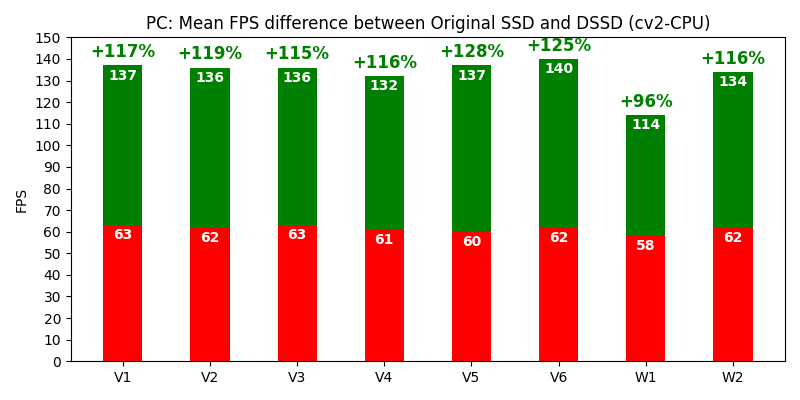
\includegraphics[width = \linewidth]{Mean Difference FPS pc only CPU.png}
                \centering
                \vspace{-0.7cm} 
                \caption{{\bfseries{\emph{Macbook Pro (OpenCV - CPU)}}}}
            \end{figure}
        \end{minipage}
        \begin{minipage}{0.45\linewidth}
            \begin{figure}
                \centering
                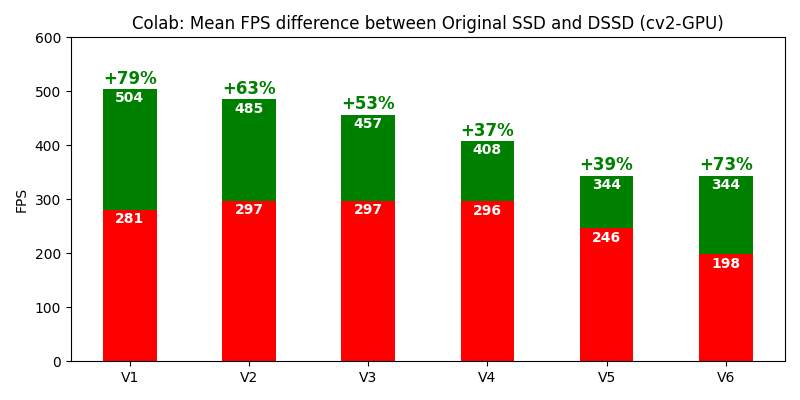
\includegraphics[width = \linewidth]{Mean Difference FPS Colab only GPU.png}
                \centering
                \vspace{-0.7cm} 
                \caption{{\bfseries{\emph{Google Colab (OpenCV - GPU)}}}}
            \end{figure}
        \end{minipage}
    \end{minipage}
    \footnotetext[1]{\scriptsize Sorgenti input: 6 Video (V) e 2 Webcam (W), tutti con differenti risoluzioni.}
\end{frame}
